 
\documentclass[conference]{IEEEtran}
%\IEEEoverridecommandlockouts
% The preceding line is only needed to identify funding in the first footnote. If that is unneeded, please comment it out.
\usepackage{cite}
\usepackage[ngerman]{babel}
\usepackage[utf8]{inputenc}
\usepackage{amsmath,amssymb,amsfonts}
\usepackage{algorithmic}
\usepackage{float}
\usepackage{graphicx}
\usepackage{textcomp}
\usepackage{xcolor}
\usepackage{listings}

\bibliographystyle{ieeetr}


\definecolor{pblue}{rgb}{0.13,0.13,1}
\definecolor{pgreen}{rgb}{0,0.5,0}
\definecolor{pred}{rgb}{0.9,0,0}
\definecolor{pgrey}{rgb}{0.46,0.45,0.48}
\lstset{language=Java,
	showspaces=false,
	showtabs=false,
	breaklines=true,
	tabsize=2,
	showstringspaces=false,
	breakatwhitespace=true,
	commentstyle=\color{pgreen},
	keywordstyle=\color{pblue},
	stringstyle=\color{pred},
	basicstyle=\ttfamily
}


\usepackage{url}
\def\BibTeX{{\rm B\kern-.05em{\sc i\kern-.025em b}\kern-.08em
    T\kern-.1667em\lower.7ex\hbox{E}\kern-.125emX}}
\begin{document}

\title{Medizinische Bildverarbeitung - Optical Imaging}

\author{\IEEEauthorblockN{Eldin Ramic, Alexander Straube}
\IEEEauthorblockA{\textit{Hochschule München} \\
München, Deutschland \\
e.ramic@hm.edu, straube@hm.edu}
}

\maketitle

\section{Aufgabenstellung}
Ziel der Aufgabe ist es die optischen Bilddaten eines flexiblen Endoskops einzulesen, aufzubereiten und darzustellen. Die Bilddaten bestehen aus einem Farb- und einem korrespondieren Fluoreszenzbild. Zur Lösung der Aufgabe soll selbständig geeigneter Quellcode erstellt werden. Die Programmiersprache Python wurde zur Lösung aller Teilaufgaben verwendet.

\section{Datensatz}
Die Bilddaten liegen im FITS Dateisystem vor (http://fits.gsfc.nasa.gov/). Dieses Bilddateisystem ist in der Wissenschaft vor allem in der Astronomie verbreitet und zeichnet sich durch große Vielseitigkeit aus (Meta Informationen, hochdimensionale Datenwürfel...).

\section{Einfache Überlagerung}
Hierbei sollen die Farbbilder und die Fluoreszenzbilder überlagert werden. Diese müssen zunächst eingelesen und gemäß der Zeitstempel zeitlich zugeordnet werden. Die Zeitstempel der Bildaufnahmen lassen sich aus den Metadaten der Bilder entnehmen. Anschließend werden die Bilder mithilfe der gespeicherten Registrierungsparametern (aus den Metadaten) koregistriert . 

\subsection{Einlesen der Bilddaten}
Zum Einlesen der Bilddaten wird das Modul \textit{fits} aus der Bibliothek \textit{astropy.io} verwendet.

\subsection{Zeitliche Zuordnung}
Die Zeitstempel der einzelnen Bilder werden aus den Metadaten herausgelesen. Für die zeitliche Zuordnung wird das folgende Verfahren angewendet: \\

a) Lese Zeitstempel aus den Metadaten des jeweiligen Farbbildes $I_n$ ab.

b) Finde das Fluoreszenzbild mit der geringsten absoluten Differenz zwischen dem Zeitstempel des Fluoreszenzbildes und des Farbbildes $I_n$.

c) Wiederhole das Verfahren für alle weiteren Farbbilder

\subsection{Koregistrierung}
Vor der Transformation werden die Fluoreszenznilder auf die Größe der Farbbilder skaliert.
Die jeweils neun Registrierungsparameter werden aus den Metadaten herausgelesen (TRANSC0, ..., TRANSC8). \\

Dadurch ergibt sich die Transformationsmatrix M: \\

M = 
$\begin{bmatrix}
 TRANSC0 & TRANSC1 & TRANSC2 \\
 TRANSC3 & TRANSC4 & TRANSC5 \\
 TRANSC6 & TRANSC7 & TRANSC8 \\
\end{bmatrix}$ \\

Zusätzlich werden die Fluoreszenzbilder binarisiert und die einzelnen Ausreißer durch eine mehrstufige Erosion entfernt. \\

Ein Beispiel für ein korrespondierendes Bildpaar:

\begin{figure}[h]
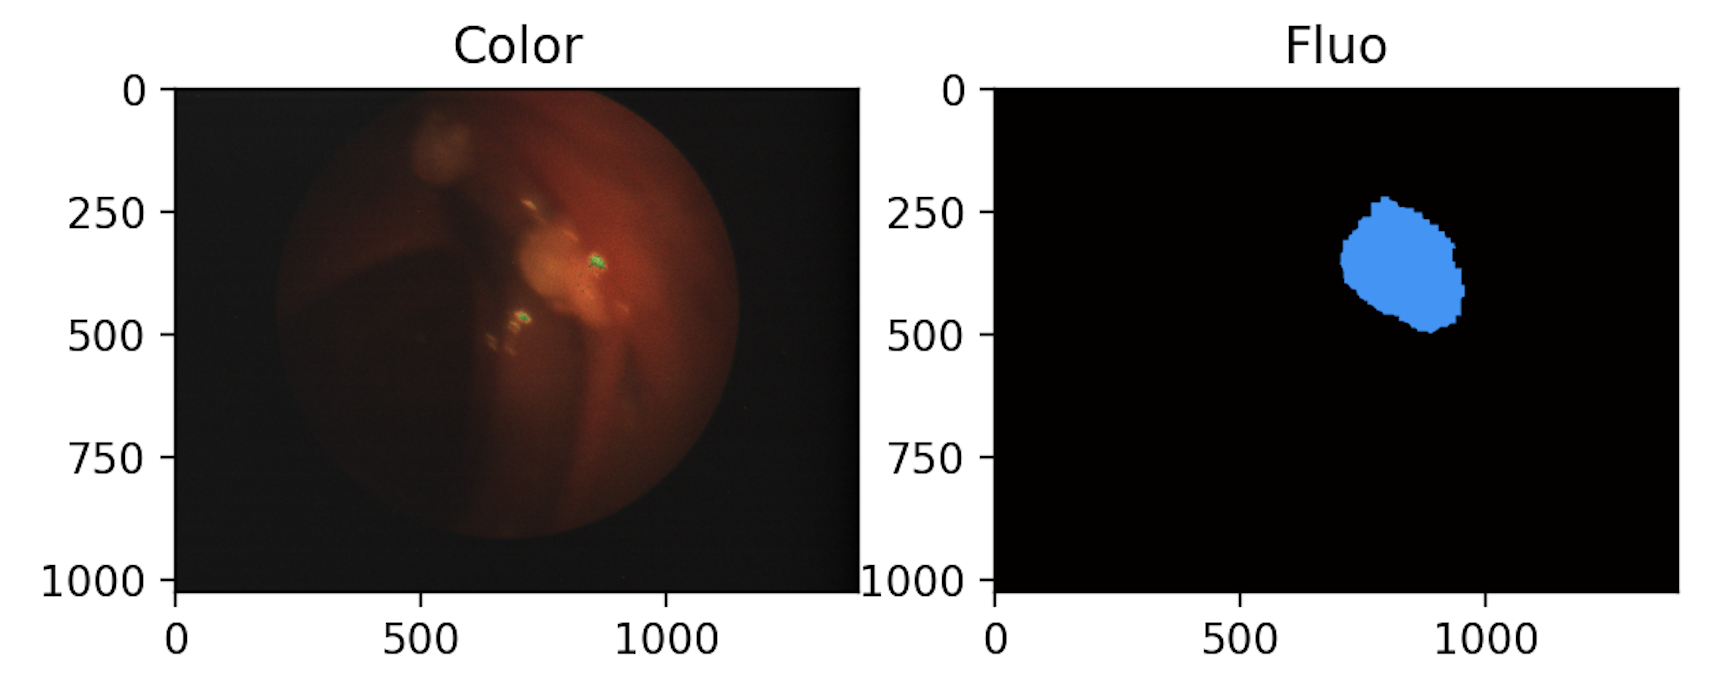
\includegraphics[width=8cm]{Fig1}
\caption{links: Farbbild; rechts: Fluoreszenzbild}
\end{figure}


\subsection{Überlagerung}

Ein Beispiel für eine Überlagerung eines korrespondierenden Bildpaares:

\begin{figure}[h]
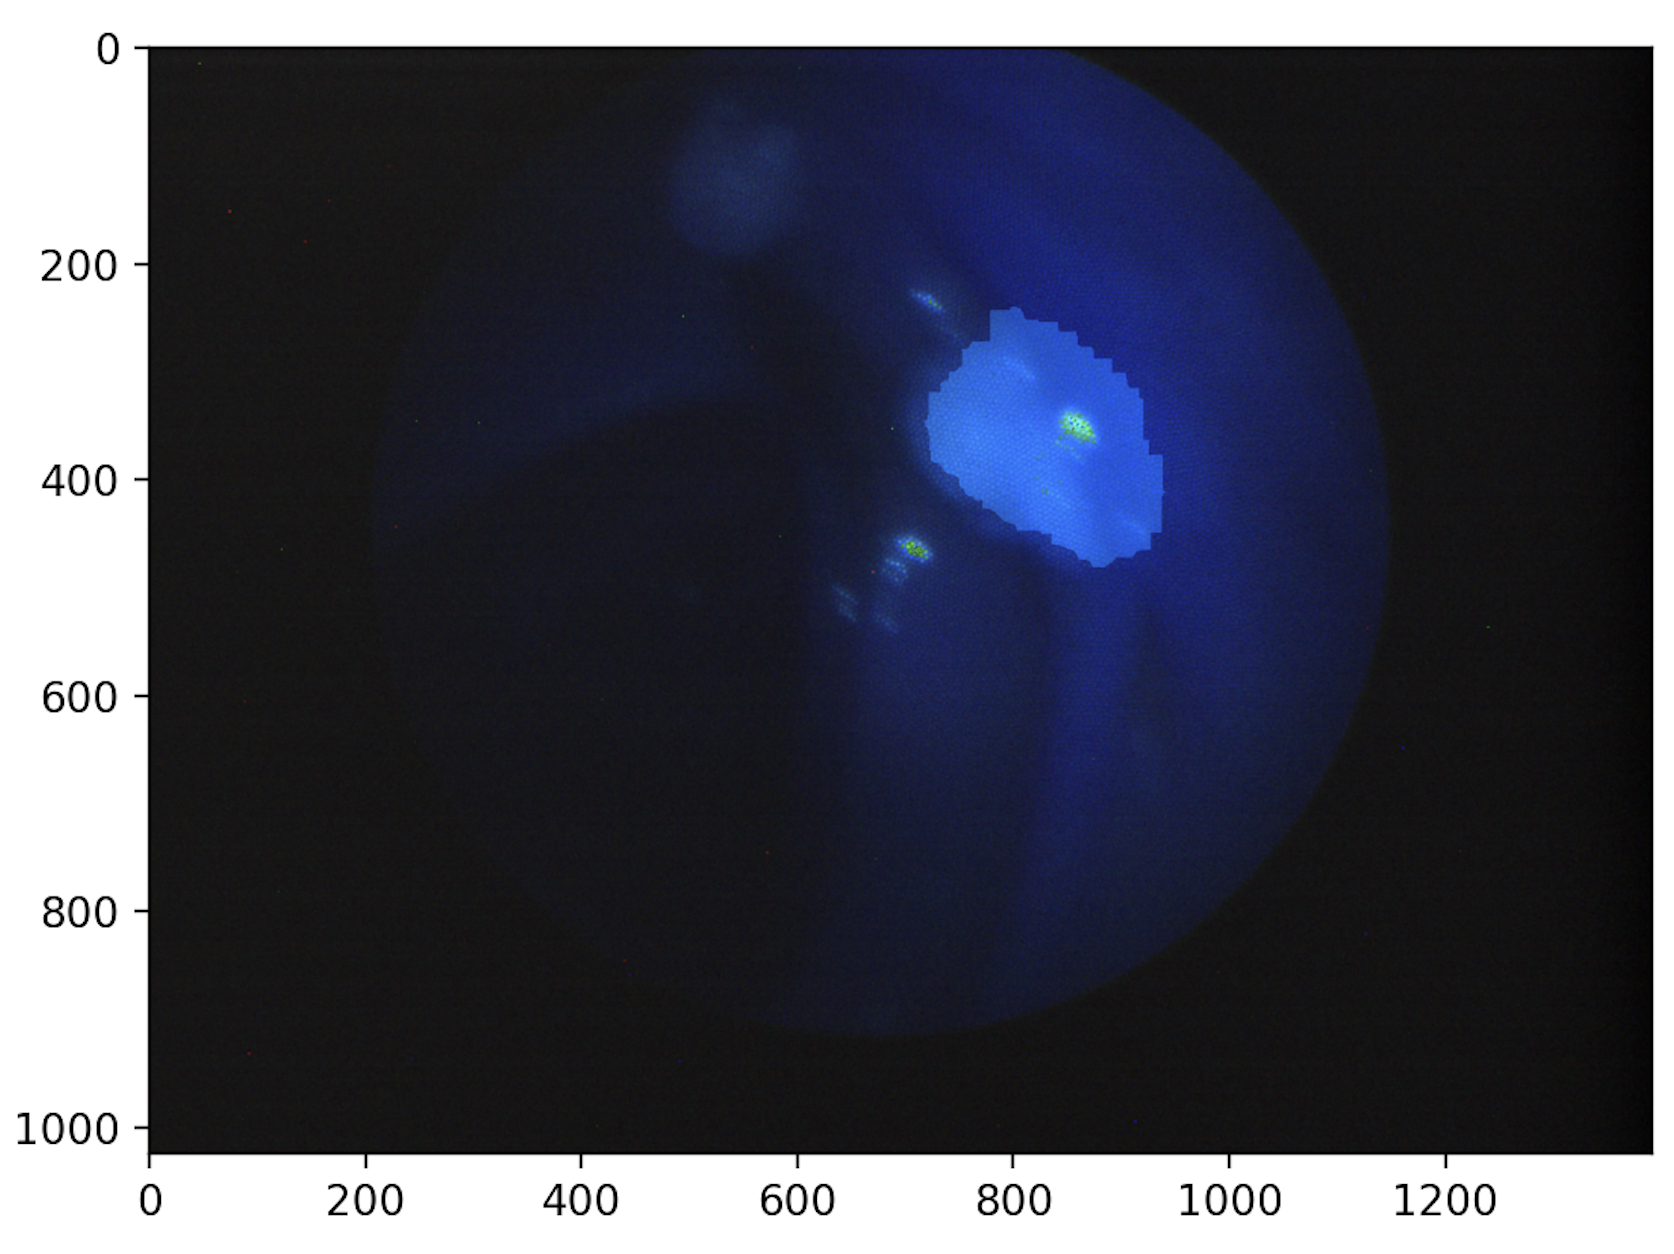
\includegraphics[scale=0.22]{Fig2}
\caption{Überlagertes Bild}
\end{figure}

\section{Erstellen eines hochaufgelösten überlagerten Falschfarbenvideos} 

Hierbei sollen die Reflektionsdaten aus einer Videodatei (.mp4) eingelesen und mit den korrespondierenden Fluoreszenzbildern überlagert werden. Eine geeignete adaptive Methode zur Bestimmung der Registrierungsparameter (in Ort und Zeit) ist hier nötig. \\

\textbf{Idee: Bestimme die zugehörige Konturen und berechne anhand der Kontur-Mittelpunkte die Transformationsmatrix} \\

\subsection{Vorverarbeitung}

Für diesen Aufgabenteil werden die vorverarbeiteten Fluoreszenzbilder aus der vorherigen Aufgabe übernommen. \\

Da der Bilddatensatz der Reflektionsdaten deutlich größer ist als der der Fluoreszenzbildern, muss dieser zunächst angepasst werden. Dabei werden einzelne Fluoreszenzbilder mehrfach dem Bilddatensatz beigefügt, sodass die Größen der Bilddatensätze übereinstimmen. \\

Bevor die Konturen berechnet werden, wird die Auflösung beider Bilddatensätze zur Reduzierung des Berechnungsaufwandes auf 480x480 Pixel reduziert. Zudem werden auch die Reflektionsbilder binarisiert, um die Anzahl der falschen Konturen zu reduzieren. 

\subsection{Ansatz}

Das Ziel ist, die passende Kontur in beiden korrespondierenden Bildern zu bestimmen und den Kontur-Mittelpunkt zu berechnen. Denn mithilfe der Mittelpunktskoordinaten kann die jeweilige Transformationsmatrix bestimmt werden. In diesem Fall wird eine Affine-Transformation durchgeführt. Da die Größen der Konturen ungefähr übereinstimmen, wird mit der Transformation lediglich die Kontur anhand des Zentrums in Richtung der x- und y-Achse verschoben. Die Verschiebungen werden wie folgt berechnet: \\

$(x_s/y_s)$: Verschiebung \\
$(x_1/y_1)$: Mittelpunkt (Reflexionsdaten) \\
$(x_2/y_2)$: Mittelpunkt (Fluoreszenzbilder) \\

\begin{equation}
  \begin{aligned}
    x_s = x_1 - x_2\\
      y_s = y_1 - y_2\\ \\
  \end{aligned}
\end{equation}


Da es sich hierbei nur um eine Verschiebung auf der x- und y-Achse handelt, kann man die Matrix bzw. die neuen Pixel-Koordinaten wie folgt berechnen: \\ \\ \\

Affine Transformation: 

\begin{equation}
  \begin{aligned}
\begin{pmatrix} x' \\ y' \end{pmatrix} = 
\left(\begin{array}{ccc} 1 & 0 & x_s \\ 0 & 1 & y_s \end{array}\right)
\left(\begin{array}{r} x_1 \\ y_1 \\ 1 \end{array}\right) 
  \end{aligned}
\end{equation}

$(x'/y')$ stellt dabei die transformierte Koordinate dar.


\subsection{Weitere Maßnahmen}

Des Weiteren werden folgende Maßnahmen zur Detektion der korrekten Kontur innerhalb der Reflektionsbilder getroffen: \\

\textbf{- Bereichseingrenzung:} Im gesamten Bilddatensatz lässt sich das Bild auf die linke-obere Bildhälfte reduzieren, da die korrekte Kontur nur innerhalb dieser sich befindet. \\

\textbf{- Iterative Helligkeitserhöhung:} In einigen Fällen werden alle Konturen heraus-binarisiert. Dies kommt vor, wenn das Bild vergleichsweise dunkel ist und die Binarisierung in der Vorverarbeitung nicht optimal gewählt ist. Diesem wird entgegengesteuert, indem die Helligkeit iterativ erhöht wird, bis eine Kontur ermittelt werden kann.  \\

\subsection{Ergebnis}

In den meisten Fällen werden die Bilder korrekt überlagert. Nichtsdestotrotz kommt es an manchen Stellen vor, dass die falsche Kontur als 'einzige' Kontur bestimmt wird und somit die Transformation nicht korrekt durchgeführt wird. Außerdem hat sich Bereichseingrenzung als positiv erwiesen, da dabei immer die korrekte Kontur zur Bestimmung der Transformationsmatrix gewählt wurde.

\end{document}